\documentclass{article}

\usepackage[utf8]{inputenc}
\usepackage[provide=*,french]{babel}
\usepackage[numbers]{natbib}
\usepackage{hyperref}
\usepackage{graphicx}
\usepackage{amsmath,amssymb,amsthm}
\usepackage{enumitem}
\usepackage{geometry}
\geometry{left = 1in, right = 1in, top = 1in, bottom=1in}

\usepackage{tikz}
\usetikzlibrary{bayesnet}

\usepackage{subcaption}


\usepackage{listings}
\usepackage{xcolor}  

\title{Implémentation et validation de réseaux bayésiens dynamiques d'ordre T avec pyagrum}
\author{Jad CHAMSEDDINE \and Jesus Alejandro GOMEZ URZUA}

\setlength{\parindent}{0pt}
\setlength{\parskip}{0.8em}

\newcommand\independent{\perp\!\!\!\!\!\!\perp} 

\lstset{
  basicstyle=\ttfamily\small,
  keywordstyle=\color{blue},
  commentstyle=\color{gray},
  stringstyle=\color{orange},
  breaklines=true,
  frame=single,
  numbers=left,
  numberstyle=\tiny\color{gray},
  showstringspaces=false,
  tabsize=2,
  language=Python  
}

\begin{document}
\maketitle

\setcounter{tocdepth}{2}
\tableofcontents

\section{Introduction}


Les réseaux bayésiens (BN) constituent un cadre formel puissant pour la représentation de connaissances et le raisonnement
probabiliste. Ils modélisent des relations de dépendance conditionnelle entre variables aléatoires au moyen d'un graphe
orienté acyclique associé à une factorisation de la probabilité jointe. En intelligence artificielle, ils sont utilisés
avec succès dans des domaines aussi variés que la classification d'échantillons biologiques\cite{doi:10.1021/jf9013235}
la modélisation du risque en agriculture\cite{BRESSAN2009579} ou encore l'analyse de systèmes de sécurité
industrielle\cite{KANNAN2007255}.

Les réseaux bayésiens dynamiques (dBN), étendent ce cadre aux processus temporels en modélisant l'évolution des variables
au cours du temps. Cette extension permet de représenter des phénomènes dynamiques tout en conservant les propriétés de
factorisation des BN classiques. De nombreuses applications en séquençage, reconnaissance vocale ou séries temporelles
motivent leur étude. \cite{perrin2003gene, zweig1998speech}

Dans ce contexte, la bibliothèque \texttt{pyagrum} fournit un cadre de développement en Python pour la modélisation et
l'inférence dans les réseaux bayésiens. Si elle offre déjà un support partiel pour les réseaux dynamiques d'ordre 2
(2TBN), elle ne propose pas de mécanisme général pour la représentation ou l'apprentissage de modèles dynamiques d'ordre
arbitraire $K$.

Le travail présenté dans ce rapport s'inscrit dans le cadre de l'UE LU2IN013, mené en binôme sous la direction de
Pierre-Henri WUILLEMIN, et visant à étendre les fonctionnalités de \texttt{pyagrum} pour prendre en charge les réseaux
bayésiens dynamiques d'ordre arbitraire. L'objectif principal a été la conception d'un cadre logiciel pour manipuler de
tels objets de manière efficace, ainsi que le développement de méthodes d'apprentissage adaptées à ce contexte.

Ce rapport présente de manière détaillée les résultats de ce projet. Après un rappel de l'état de l'art sur les réseaux
bayésiens et leurs extensions dynamiques, nous exposons les choix de conception et d'implémentation de la classe
\texttt{KTBN}. Nous présentons ensuite les algorithmes d'apprentissage développés, couvrant à la fois l'apprentissage
structurel, l'estimation des paramètres, et la sélection automatique de l'ordre $K$. Une évaluation expérimentale
vient conclure le rapport, illustrant les performances des approches proposées sur des données synthétiques.

\section{État de l'art}

Afin de situer le travail effectué dans un cadre théorique rigoureux, cette section présente les principaux concepts
utilisés au cours du projet. Nous introduisons d'abord les réseaux bayésiens. Nous abordons ensuite leur extension
temporelle, les réseaux bayésiens dynamiques (dBN). Enfin, nous évoquons brièvement les approches classiques
d'apprentissage structurel.

\subsection{Réseaux Bayésiens : Concepts Essentiels}


Un réseau bayésien (BN) est un modèle graphique probabiliste représenté par un graphe dirigé sans circuit
(DAG) \cite{mihajlovic2001dynamic}, où les nœuds correspondent à des variables aléatoires, et les arcs codent
des relations de dépendance probabilistes ou causales.

Sous une interprétation purement statistique, un BN constitue une représentation compacte des relations
d'indépendance conditionnelle présentes dans les données d'observation et peut être utilisé pour l'inférence des
distributions conditionnelles et marginales. Si l'on adopte une interprétation causale, le BN devient un réseau
bayésien causal (CBN), un DAG unique qui permet de raisonner sur les interventions et de mieux comprendre les
mécanismes sous-jacents du système modélisé. Dans ce cadre, la relation $A \to B$ signifie que $A$ est une cause
directe de $B$.

En termes de structure, un nœud $A$ est appelé parent d'un nœud $B$ si une arc $A \to B$ existe, et réciproquement,
$B$ est un enfant de $A$. L'absence d'un arc entre deux nœuds implique une indépendance conditionnelle entre ces
variables, étant donné leurs parents respectifs. Cette propriété est formalisée par la propriété de Markov locale :

\begin{center}
    Toute variable $X_i$ est indépendante de ses non-descendants, sachant ses parents directs.
\end{center}

Un réseau bayésien encode une décomposition factorisée de la loi de probabilité jointe en exploitant la structure
du DAG. Plus précisément, étant donné un ensemble de variables aléatoires $X_1, X_2, \dots, X_n$ organisées selon
la topologie du DAG, la probabilité jointe se factorise comme suit :

$$
    \mathbb{P}(X_1, X_2, \dots, X_n) = \prod_{i=1}^{n} \mathbb{P}(X_i \mid \text{Parents}(X_i))
$$

où $\text{Parents}(X_i)$ désigne l’ensemble des parents de la variable $X_i$ dans le graphe.

Par exemple, considérons une factorisation donnée par :

$$
    \mathbb{P}(X, Y, Z) = \mathbb{P}(X) \mathbb{P}(Y \mid X) \mathbb{P}(Z \mid X).
$$

Le graphe correspondant à cette décomposition est un DAG de la forme :

\begin{center}
    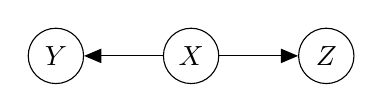
\begin{tikzpicture}[every node/.style={latent}]
        \node (X) {$X$};
        \node (Y) [left=of X] {$Y$};
        \node (Z) [right=of X] {$Z$};
        \edge {X}{Y};
        \edge {X}{Z};
    \end{tikzpicture}
\end{center}


L'analyse des relations d'indépendance conditionnelle dans un réseau bayésien repose sur le critère de
d-séparation \cite{10.5555/534975}. Soient $X, Y, Z$ trois ensembles disjoints de nœuds d'un DAG $\mathcal{G}$.
L'ensemble $Z$ est dit d-séparateur de $X$ et $Y$, noté $\langle X \mid Z \mid Y \rangle_d$, si et seulement si
tout chemin non dirigé entre un nœud de $X$ et un nœud de $Y$ est bloqué par $Z$. Un chemin est dit bloqué s'il
existe un nœud $W$ sur ce chemin vérifient l'une des deux conditions suivantes : $W$ est un nœud en collision,
c'est-à-dire qu'il existe dans $\mathcal{G}$ deux arcs entrants vers $W$ le long du chemin considéré,
autrement dit une structure de la forme $A \to W \gets B$, et qu'aucun nœud parmi $W$ et ses descendants n'appartient
à $Z$, ou bien, $W$ n'est pas un nœud en collision et $W$ appartient à $Z$.

Cette caractérisation graphique implique l'indépendance conditionnelle dans l'espace probabiliste :

$$
    Z \text{ d-sépare } X \text{ et } Y \implies X \independent Y | Z
$$

\subsection{Apprentissage des BN}

L'apprentissage d'un réseau bayésien à partir de données est un problème NP-difficile. Cela a été prouvé par
\citet{chickering1996learning}. Cette complexité provient de l'explosion du nombre de structures possibles,
qui croît exponentiellement avec le nombre de variables. Malgré cette complexité inhérente, plusieurs approches
heuristiques ont été développées pour approximer la solution optimale.

\subsubsection{Classes d'Équivalence de Markov}


Dans un réseau bayésien, la structure d'un DAG encode un ensemble d'indépendances conditionnelles à travers le
critère de d-séparation. Toutefois, une même distribution de probabilités peut être représentée par plusieurs
DAGs distincts qui induisent exactement les mêmes relations d'indépendance conditionnelle. Cette propriété
conduit à la notion de classe d'équivalence de Markov:

\begin{center}
    Deux DAGs $\mathcal{G}_1$ et $\mathcal{G}_2$ sont dits Markov-équivalents si et seulement si ils induisent le
    même ensemble d'indépendances conditionnelles.
\end{center}

\begin{figure}
    \centering
    \begin{minipage}[b]{0.6\textwidth}
        \centering
        \begin{subfigure}[b]{\textwidth}
            \centering
            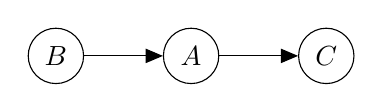
\begin{tikzpicture}[every node/.style={latent}]
                \node (B) {$A$};
                \node (A) [left=of B] {$B$};
                \node (C) [right=of B] {$C$};
                \edge {A}{B};
                \edge {B}{C};
            \end{tikzpicture}
            \caption{}
        \end{subfigure}
        \vspace{0.8em}
        \begin{subfigure}[b]{\textwidth}
            \centering
            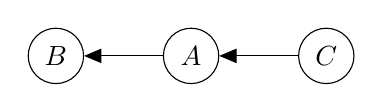
\begin{tikzpicture}[every node/.style={latent}]
                \node (B) {$A$};
                \node (A) [left=of B] {$B$};
                \node (C) [right=of B] {$C$};
                \edge {B}{A};
                \edge {C}{B};
            \end{tikzpicture}
            \caption{}
        \end{subfigure}
        \vspace{0.8em}
        \begin{subfigure}[b]{\textwidth}
            \centering
            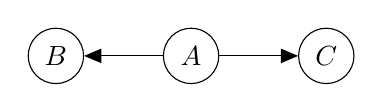
\begin{tikzpicture}[every node/.style={latent}]
                \node (B) {$A$};
                \node (A) [left=of B] {$B$};
                \node (C) [right=of B] {$C$};
                \edge {B}{A,C};
            \end{tikzpicture}
            \caption{}
        \end{subfigure}
    \end{minipage}
    \hfill
    \begin{minipage}[b]{0.35\textwidth}
        \centering
        \begin{subfigure}[b]{\textwidth}
            \centering
            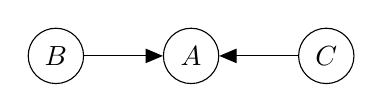
\begin{tikzpicture}[every node/.style={latent}]
                \node (B) {$A$};
                \node (A) [left=of B] {$B$};
                \node (C) [right=of B] {$C$};
                \edge {A}{B};
                \edge {C}{B};
            \end{tikzpicture}
            \caption{}
        \end{subfigure}
    \end{minipage}
    \caption{Configurations d'orientation des arêtes entre $A$, $B$ et $C$. (a)-(c) sont équivalentes ; (d) est une v-structure.}
    \label{fig:v_structure}
\end{figure}


Un élément clé dans l'analyse des classes d'équivalence est la notion de structure en V (v-structure).
Soient $A$, $B$ et $C$ trois variables représentées par des sommets dans un DAG $\mathcal{G}$. Supposons que deux
arcs relient A et B, et C et B (dans un sens ou dans l'autre), mais qu'aucun arc ne relie directement A et C.
Dans ce cas, il existe exactement quatre configurations possibles pour l'orientation des arcs entre ces trois
sommets, illustrées dans la Figure \ref{fig:v_structure}. D'un point de vue probabiliste, les trois premières configurations sont
indistinguables en ce qu'elles encodent exactement la même relation d'indépendance conditionnelle, à savoir

$$
    A \independent C \mid B.
$$

En revanche, la quatrième configuration se distingue des autres, car elle encode une relation d'indépendance différente,
en particulier

$$
    A \not\independent C \mid B.
$$

Dans cette dernière structure, le nœud $B$ possède deux arcs entrants, et il n'existe d'arc entre $A$ et $C$. Une
telle configuration est appelée une v-structure.

Le théorème de caractérisation de Verma et Pearl \cite{10.5555/534975} établit un critère nécessaire et suffisant
pour que deux DAGs soient Markov-équivalents. Deux DAGs $\mathcal{G}_1$ et $\mathcal{G}_2$ sont Markov-équivalents
si et seulement si ils vérifient simultanément les deux conditions suivantes :

\begin{enumerate}[label=(\roman*)]
    \item $\mathcal{G}_1$ et $\mathcal{G}_2$ possèdent le même squelette, c'est-à-dire qu'ils admettent
          le même graphe non orienté sous-jacent, où seules les connexions entre variables sont considérées,
          indépendamment de l'orientation des arêtes.
    \item $\mathcal{G}_1$ et $\mathcal{G}_2$ contiennent exactement les mêmes v-structures
\end{enumerate}


Ces deux conditions garantissent que les DAGs appartenant à une même classe d'équivalence induisent exactement
les mêmes relations d'indépendance conditionnelle, et sont par conséquent indiscernables d'un point de vue
probabiliste. Il en résulte qu'un algorithme d'apprentissage statistique ne peut pas différencier deux réseaux
bayésiens issus de la même classe d'équivalence. En effet, ils sont statistiquement équivalents vis-à-vis de
l'information accessible dans les observations.

\subsubsection{Approches Basées sur les Contraintes}


Les méthodes d'apprentissage structurel basées sur les contraintes (\textit{constraint-based structure learning})
s'appuient sur l'identification des indépendances conditionnelles entre variables afin de reconstruire la
structure d'un réseau bayésien. Ces méthodes exploitent le fait que la structure d'un DAG Markov-compatible avec
une distribution de probabilités est entièrement caractérisée par les relations d'indépendance conditionnelle
entre variables.

L'algorithme suit généralement trois phases successives :

\begin{enumerate}
    \item Construction du squelette

          On détermine d'abord le squelette du graphe, c'est-à-dire son graphe sous-jacent non orienté,
          en effectuant des tests d'indépendance conditionnelle sur les données. Deux variables sont
          reliées par une arête dans le squelette si et seulement si elles ne sont pas indépendantes
          conditionnellement à un sous-ensemble approprié des autres variables observées. Cette phase
          fournit une première approximation de la structure du réseau sans information directionnelle.

    \item Orientation des v-structures

          Une fois le squelette obtenu, il est nécessaire d'identifier et d'orienter les v-structures,
          qui sont les seules configurations dont l'orientation est déductible directement à partir des
          relations d'indépendance conditionnelle observées. Ces orientations sont imposées de manière
          unique afin de préserver les relations d'indépendance et de dépendance induites par les tests effectués.

    \item Orientation des arêtes restantes

          Après l'identification des v-structures, les autres arêtes du graphe doivent être orientées en
          respectant deux contraintes fondamentales :
          \begin{enumerate}[label=(\roman*)]
              \item éviter la formation de cycles dirigés, et
              \item ne pas introduire de nouvelles v-structures non justifiées par les indépendances
                    conditionnelles observées.
          \end{enumerate}


          Pour cela, des règles d'orientation supplémentaires sont appliquées de manière itérative, comme la
          propagation des orientations dérivées des relations d'indépendance.
\end{enumerate}

L'exactitude de ces méthodes dépend fortement de la fiabilité des tests d'indépendance, qui peuvent être
affectés par le bruit ou la taille limitée des échantillons. Dans certains cas, elles ne permettent pas d'orienter
toutes les arêtes, ce qui conduit à l'obtention d'un DAG partiellement orienté (\textit{partially directed acyclic graph},
PDAG), représentant l'ensemble des structures Markov-équivalentes compatibles avec les données.

\subsubsection{Approches Basées sur les Scores}

Les méthodes basées sur les scores (\textit{score-based}) modélisent l'apprentissage de la structure comme un
problème d'optimisation : il s'agit de trouver la structure qui maximise un score mesurant l'adéquation du
modèle aux données. Parmi les scores les plus couramment utilisés figurent le BIC (\textit{Bayesian Information Criterion}),
le BDe (\textit{Bayesian Dirichlet equivalent}) et le MDL (\textit{Minimum Description Length}).

Ces scores équilibrent deux objectifs contradictoires : obtenir un bon ajustement aux données observées tout en
pénalisant les structures trop complexes, afin d'éviter le sur-apprentissage.

Dans la pratique, la recherche de la structure optimale est rendue difficile par la taille exponentielle de l'espace
des graphes possibles. Les algorithmes utilisés sont donc généralement gloutons (greedy), explorant l'espace des
DAGs à l'aide d'ajouts, suppressions ou inversions d'arcs qui améliorent localement le score.

\subsection{Réseaux Bayésiens Dynamiques}

Les réseaux bayésiens dynamiques (dBN) constituent une extension naturelle des réseaux bayésiens aux processus
évolutifs, où les variables aléatoires sont observées sur plusieurs instants successifs. Ils permettent de modéliser
des systèmes dynamiques probabilistes, dans lesquels les dépendances statistiques entre les variables évoluent dans
le temps de manière structurée.

Les dBN s'appuient généralement sur l'hypothèse de Markov d'ordre 1, c'est-à-dire que l'état du système à l'instant
$t+1$ ne dépend que de son état à l'instant $t$. Cette approche inclut notamment les \textit{2-Time-slice Bayesian Networks}
(2TBN), déjà présents dans \texttt{pyagrum}.

Dans le cadre de notre projet, nous considérons une généralisation de ce modèle, les réseaux bayésiens dynamiques d'ordre $K$
(KTBN), dans lesquels la dynamique temporelle du système repose sur les $K-1$ dernières tranches temporelles. Plus
formellement, un KTBN se compose de deux parties :

\begin{enumerate}
    \item Une structure initiale décrivant la distribution jointe des variables sur les $K-1$ premières tranches
          temporelles $(X^{(0)}, X^{(1)}, \dots, X^{(K-2)})$, modélisée par un réseau bayésien classique ;
    \item Un modèle de transition qui encode la distribution conditionnelle
          $\mathbb{P}(X^{(t)} \mid X^{(t-1)}, \dots, X^{(t-(K-1))})$ pour tout $t \geq K$, sous l'hypothèse
          que cette transition reste stationnaire au cours du temps.
\end{enumerate}

Ce modèle repose donc sur deux hypothèses fondamentales :

\begin{enumerate}
    \item Hypothèse de Markov d'ordre $K-1$ : l'état futur dépend uniquement des $K-1$ derniers états passés ;
    \item Stationnarité de la transition : la loi de transition est identique pour $t \geq K$, ce qui permet
          de réutiliser la même structure temporelle à chaque pas.
\end{enumerate}

En pratique, la représentation graphique d'un KTBN peut être réalisée au moyen d'un seul DAG statique, dans
lequel chaque nœud représente une variable à un instant donné. Une fois les $K-1$ premières tranches temporelles
définies, la $K$-ième est utilisée comme patron de transition, qui peut être "déroulé" de manière répétée pour
modéliser un processus de longueur arbitraire.

Malgré la expressivité du modèle KTBN, celui-ci reste relativement peu exploré dans la littérature. En dehors
de cas particuliers bien étudiés, tels que les modèles de Markov cachés ou les 2TBN, peu de travaux portent
sur la modélisation de réseaux bayésiens dynamiques d'ordre $K$ arbitraire. En particulier, les questions liées
à l'apprentissage automatique de ces structures demeurent encore ouvertes.

Dans ce contexte, nous explorons des méthodes pour l'apprentissage structurel d'un KTBN à ordre $K$ fixé,
ainsi que pour l'estimation de cet ordre à partir des données. Les algorithmes que nous proposons s'appuient sur
des critères d'adéquation statistique, tels que le score BIC.



\section{Modélisation et implantation de la structure KTBN}

\subsection{Objectif de la classe \texttt{KTBN}}

La bibliothèque \texttt{pyagrum} prend en charge les réseaux bayésiens statiques et propose un support partiel
pour les 2TBN. Elle ne permet toutefois pas de représenter ou manipuler directement des réseaux bayésiens
dynamiques d'ordre $K$ quelconque.

La classe \texttt{KTBN} a pour objectif d'étendre cette fonctionnalité en introduisant une surcouche au-dessus
d'un objet \texttt{BayesNet}. Cette abstraction gère explicitement la structure temporelle du modèle, permettant
notamment l'accès aux variables temporelles, la manipulation d'arcs inter-tranches et la génération de trajectoires,
tout en restant compatible avec l'infrastructure de \texttt{pyagrum}.


\subsection{Architecture et conception de la classe \texttt{KTBN}}

\subsubsection{Classe d'abstraction et encapsulation}

La classe \texttt{KTBN} enveloppe un réseau bayésien standard de pyagrum (\texttt{gum.BayesNet}) dans une classe
adaptée aux réseaux bayésiens dynamiques. Cette approche offre plusieurs avantages :

\begin{itemize}
    \item Exploitation des fonctionnalités existantes :  L'utilisation d'un \texttt{gum.BayesNet} sous-jacent
          permet de bénéficier de toutes les fonctionnalités robustes et optimisées de \texttt{pyagrum} (inférence,
          apprentissage, manipulation des CPT, etc.).
    \item Compatibilité : La possibilité de convertir un \texttt{KTBN} vers un réseau bayésien standard via
          la méthode \texttt{to\_bn()} permet de réutiliser les fonctionnalités de \texttt{pyagrum}.
    \item Abstraction temporelle : La classe \texttt{KTBN} masque la complexité interne et propose des méthodes
          simples pour les opérations temporelles.
\end{itemize}


\subsubsection{Distinction entre variables temporelles et atemporelles}

Un point clé de notre implémentation est de séparer deux types de variables :

\begin{itemize}
    \item Variables temporelles : Variables qui changent selon le temps. Pour un ordre $K$, chaque variable
          temporelle est copiée $K$ fois dans le réseau bayésien.
    \item Variables atemporelles : Variables qui restent fixes dans le temps.
\end{itemize}

Deux ensembles internes permettent cette séparation :

\begin{lstlisting}
    self._temporal_variables = set()     # Variables temporelles
    self._atemporal_variables = set()    # Variables atemporelles
\end{lstlisting}


\subsubsection{Système d'encodage des noms de variables}

Pour différencier les variables dans le temps, chaque variable temporelle reçoit un nom unique composé de son nom
original, d'un délimiteur (\# par défaut)  et du time-slice correspondant. Par exemple, \texttt{Temperature\#0},
\texttt{Temperature\#1}, \texttt{Humimidity\#2}. Les variables atemporelles gardent leur nom original. Cette méthode
permet d'identifier chaque variable à un moment précis.

Les fonctions \texttt{encode\_name()} et \texttt{decode\_name()} permettent la conversion entre la représentation
logique (nom et time-slice séparés) et la représentation technique (nom encodé) :

\begin{lstlisting}    
    def encode_name(self, variable: str, time_slice: int) -> str:
    # Convertit (nom, time-slice) en nom_technique
    
    def decode_name(self, name: str) -> Tuple[str, int]:
    # Convertit nom_technique en (nom, time-slice)
\end{lstlisting}



\subsection{Méthodes de base et interface}

\subsubsection{Adaptation de l'API \texttt{pyagrum}}

Dans \texttt{pyagrum}, les variables sont manipulées à l'aide de méthodes avec des paramètres simples du type
\texttt{méthode(nom\_variable)}. Cependant, dans un réseau bayésien dynamique, chaque variable est indexée par son
time-slice, ce qui nécessite une désambiguïsation temporelle lors de la manipulation.

La classe \texttt{KTBN} introduit ainsi une interface adaptée, dans laquelle les méthodes attendent un couple
\texttt{(nom\_variable, time\_slice)} comme paramètre, sous la forme \texttt{méthode(nom\_variable, time\_slice)},
avec la convention $t=-1$ pour les variables atemporelles.

Cette extension permet d'ajouter des arcs entre différentes tranches temporelles, par exemple :

\begin{lstlisting}
    ktbn.addArc(("Humidity", 1), ("Humidity", 2))
\end{lstlisting}

ce qui crée un arc de la variable \texttt{Humidity} à l'instant $t = 1$ vers la même variable à l'instant $t = 2$.

\subsubsection{Méthodes d'interaction avec \texttt{pyagrum}}

La classe KTBN expose plusieurs méthodes permettant l'interaction directe avec le réseau bayésien sous-jacent :

\begin{itemize}
    \item \texttt{addVariable(variable, temporal)} : Ajout d'une variable (temporelle ou atemporelle)
    \item \texttt{addArc(tail, head)} : Ajout d'un arc avec spécification temporelle
    \item \texttt{cpt(variable, time\_slice)} : Accès aux tables de probabilité conditionnelle (CPT)
    \item \texttt{to\_bn()} : Conversion vers un \texttt{gum.BayesNet} standard
    \item \texttt{from\_bn(bn, delimiter)}: Création d'un KTBN à partir d'un réseau bayésien existant
\end{itemize}

Ces méthodes permettent de modifier et d'accéder au réseau bayésien sous-jacent tout en respectant les contraintes
temporelles et la logique de la classe \texttt{KTBN}.


\subsubsection{Méthodes spécifiques aux réseaux dynamiques}

Au-delà de l'adaptation de l'interface de \texttt{pyagrum} à la temporalité, la classe \texttt{KTBN} introduit
plusieurs méthodes spécifiques aux réseaux bayésiens dynamiques :

\begin{itemize}
    \item \texttt{unroll(n)} : méthode permettant de dérouler le \texttt{KTBN} sur $n$ tranches temporelles.
          Elle génère un BN statique équivalent, compatible avec les outils standards de
          \texttt{pyagrum}. L'algorithme :
          \begin{enumerate}
              \item duplique les variables temporelles pour chaque nouvelle tranche ;
              \item réplique la structure des arcs intra et inter-tranches selon le schéma de transition ;
              \item ajuste les CPT en conséquence.
          \end{enumerate}
    \item \texttt{sample(n\_trajectories, trajectory\_len, processes)} : génère un ensemble de trajectoires
          aléatoires à partir du modèle, en exploitant la parallélisation via le module
          \texttt{multiprocessing} de Python.
    \item \texttt{random(k, n\_vars, n\_mods, n\_arcs)} : crée un KTBN aléatoire respectant les contraintes
          structurelles imposées, pratique pour les phases de test et de validation expérimentale.
    \item \texttt{log\_likelihood(trajectories)} : calcule la log-vraisemblance d'un ensemble de trajectoires
          données, une mesure essentielle pour l'évaluation et l'apprentissage du modèle.
\end{itemize}


\subsubsection{Visualisation des KTBN}

Afin de permettre la visualisation claire et structurée des réseaux KTBN dans un environnement Jupyter, nous avons
développé un module dédié, \texttt{KTBN\_notebook}, assurant la prise en charge explicite de ces modèles.
Inspirée du module \texttt{pyagrum.lib.dynamicBN}, conçu pour organiser les variables des 2TBN par tranches temporelles,
notre classe adapte le rendu graphique aux spécificités des KTBN : elle regroupe les variables par tranche temporelle,
positionne les nœuds de manière cohérente, et distingue visuellement les variables atemporelles lorsqu'elles sont
présentes. La figure~\ref{fig:KTBN_notebook} compare ces représentations : (\subref{fig:KTBN_notebook:a}) montre un 2TBN
standard ; (\subref{fig:KTBN_notebook:b}), l'affichage par défaut d'un KTBN via les outils existants ;
(\subref{fig:KTBN_notebook:c}), le rendu structuré produit par notre adaptation.

\begin{figure}[t]
    \centering
    \begin{subfigure}[t]{0.45\textwidth}
        \centering
        \includegraphics[width=\linewidth]{img/2TBN.png}
        \caption{2TBN standard}
        \label{fig:KTBN_notebook:a}
    \end{subfigure}
    \hfill
    \begin{subfigure}[t]{0.45\textwidth}
        \centering
        \includegraphics[width=\linewidth]{img/KTBN_gum.png}
        \caption{KTBN affiché par les outils existants}
        \label{fig:KTBN_notebook:b}
    \end{subfigure}

    \vspace{1em}

    \begin{subfigure}[t]{0.6\textwidth}
        \centering
        \includegraphics[width=\linewidth]{img/KTBN.png}
        \caption{KTBN affiché par \texttt{KTBN\_notebook}}
        \label{fig:KTBN_notebook:c}
    \end{subfigure}

    \caption{Comparaison des différentes représentations graphiques d'un KTBN.}
    \label{fig:KTBN_notebook}
\end{figure}


\subsection{Choix techniques et considérations d'implémentation}

\subsubsection{Parallélisation de l'échantillonnage}

La génération de trajectoires dans un KTBN peut être parallélisée efficacement du fait de l'indépendance entre
les trajectoires. Cette propriété garantit qu'aucune synchronisation ni communication inter-processus n'est
nécessaire durant l'échantillonnage, ce qui rend le problème naturellement adapté à une exécution concurrente.
L'implémentation repose sur le module \texttt{multiprocessing} de Python, où un pool de processus est utilisé
pour répartir la génération des trajectoires. Chaque processus exécute indépendamment une fonction d'échantillonnage,
et les résultats sont collectés à l'issue de l'exécution. Cette approche permet de tirer parti des ressources
multicœurs pour réduire significativement le temps de calcul.

Chaque trajectoire est générée en deux étapes : les $K-1$ premières tranches sont échantillonnées selon la
distribution jointe du modèle, puis les tranches suivantes sont produites de manière séquentielle à l'aide du
modèle de transition. Contrairement à une approche naïve qui consisterait à dérouler intégralement le KTBN
au préalable, au prix d'une empreinte mémoire considérable, cette méthode itérative permet une consommation
mémoire faible, rendant possible l'échantillonnage de trajectoires très longues.

\subsubsection{Validation et contraintes temporelles}

La classe KTBN vérifie automatiquement la cohérence du réseau. La méthode \texttt{\_validate\_variable()} contrôle
que les variables existent, que leur type (temporelle ou atemporelle) correspond à leur utilisation, et que les
time-slices sont valides.

La classe KTBN bloque aussi la création d'arcs qui violeraient les contraintes temporelles, comme les arcs allant
du futur vers le passé. En cas d'erreur, des exceptions claires informent l'utilisateur du problème rencontré.

\subsubsection{Tests unitaires et validation}

L'implémentation de la classe \texttt{KTBN} est accompagnée d'une suite de tests unitaires conçue avec le
module standard \texttt{unittest} de Python. Ces tests couvrent les principales fonctionnalités :
initialisation, gestion des variables temporelles et atemporelles, ajout d'arcs avec vérification des contraintes
temporelles, opérations d'unrolling, sérialisation et désérialisation, conversion depuis et vers un objet
\texttt{BayesNet}, ainsi que l'accès aux CPT. Les cas testés incluent aussi bien des situations standards
que des cas d'erreur (arcs invalides, tranches hors bornes, noms absents), permettant de vérifier la conformité
de l'API à ses spécifications et la détection correcte des usages incorrects. Cette couverture garantit que
les contraintes structurelles spécifiques aux KTBN sont bien respectées, et que les erreurs sont détectées de
manière fiable.


\section{Algorithmes d'apprentissage dynamiques}

\subsection{Apprentissage structurel avec k connu}

\subsubsection{Principe algorithmique et décomposition du problème}

L'apprentissage d'un KTBN à partir d'un ensemble de trajectoires temporelles constitue un défi particulier,
car les données sont ordonnées dans le temps et les variables présentent des dépendances à travers plusieurs
time-slices. Notre approche repose sur une décomposition du problème en deux sous-problèmes plus simples~:

\begin{enumerate}
    \item Apprentissage des k premiers pas de temps : Apprentissage des relations entre variables dans les
          k premières time-slices
    \item Apprentissage de la transition : Apprentissage des relations entre l'état t+1 et les k états précédents
\end{enumerate}

Cette décomposition s'explique par le fait qu'un KTBN n'est qu'un réseau bayésien classique qui modélise la
distribution des k premiers pas de temps et de la transition. Cette perspective permet donc de réutiliser
les algorithmes d'apprentissage existants de \texttt{pyagrum} pour apprendre le KTBN.

\subsubsection{Transformation des données et construction des bases d'apprentissage}

L'implémentation de cette approche nécessite une transformation des trajectoires originales en bases de données
adaptées à l'apprentissage de réseaux bayésiens. Cette transformation est réalisée par la fonction
\texttt{\_create\_sequences()}.

Les données sont représentées sous forme de \texttt{pd.DataFrame} via la bibliothèque \texttt{pandas}, choisie
pour ses performances, sa souplesse de manipulation et sa compatibilité directe avec les fonctions d'apprentissage
de \texttt{pyagrum}.

Processus de transformation :

\begin{enumerate}
    \item Identification des types de variables :
          \begin{itemize}
              \item Variables temporelles : Variables dont les valeurs évoluent au cours du temps.
              \item Variables atemporelles : Variables qui restent fixes dans le temps, détectées automatiquement.
                    par \texttt{\_is\_atemporal()}
          \end{itemize}
    \item Génération des séquences avec décalages :
          Pour chaque variable temporelle, nous créons $K$ colonnes~: une pour la variable à l'instant présent,
          une pour la variable à l'instant précédent, et ainsi de suite jusqu'à $K$ instants. Cela permet d'avoir
          simultanément sur une même ligne les valeurs de la variable à $K$ instants consécutifs.
\end{enumerate}

Nous obtenons ainsi deux bases de données qui capturent respectivement les conditions initiales et l'évolution temporelle :

\begin{itemize}
    \item \texttt{lags} : Contient toutes les séquences de k tranches temporelles consécutives.
    \item \texttt{first\_rows} : Contient uniquement les k premières tranches de chaque trajectoire.
\end{itemize}


\subsubsection{Implémentation de la classe Learner}

La classe \texttt{Learner} sert à apprendre la structure d'un KTBN. Elle utilise deux instances
de \texttt{gum.BNLearner}, une pour chaque partie du problème.

Processus d'apprentissage avec k connu (\texttt{learn\_ktbn()}) :

\begin{enumerate}
    \item Configuration des contraintes :
          \begin{itemize}
              \item Interdiction de parents pour les variables atemporelles (contrainte \texttt{addNoParentNode}).
              \item Définition de l'ordre des tranches temporelles via \texttt{setSliceOrder}.
          \end{itemize}
    \item Apprentissage :
          \begin{itemize}
              \item \texttt{lags\_learner} : Apprentissage des arcs de transition.
              \item \texttt{first\_learner} : Apprentissage des structures internes aux $k-1$ premières tranches.
          \end{itemize}
    \item Combinaison des résultats :
          \begin{itemize}
              \item Création du réseau à partir des premières time-slices.
              \item Ajout des variables de la dernière tranche temporelle.
              \item Ajout des arcs de transition appris.
              \item Copie des CPT.
          \end{itemize}
\end{enumerate}

Cette approche permet d'exploiter les algorithmes standards de \texttt{pyagrum} tout en prenant en compte les
dépendances temporelles propres aux KTBN.

\subsubsection{Paramétrage de l’apprentissage}

La classe \texttt{Learner} reproduit l'interface de \texttt{gum.BNLearner}, ce qui permet à l'utilisateur de
configurer librement l'apprentissage d'un KTBN. Elle applique automatiquement les mêmes paramètres aux deux
learners internes (\texttt{first\_learner} et \texttt{lags\_learner}).

Fonctionnalités exposées :
\begin{itemize}
    \item Contraintes structurelles : \texttt{addMandatoryArc()}, \texttt{addForbiddenArc()}, \texttt{setPossibleEdges()}
    \item Algorithmes d'apprentissage : \texttt{useGreedyHillClimbing()}, \texttt{useMIIC()}, \texttt{useLocalSearchWithTabuList()}
    \item Scores : \texttt{useScoreBIC()}, \texttt{useScoreAIC()}, \texttt{useScoreBDeu()}, \texttt{useScoreK2()}
    \item Priors : \texttt{useBDeuPrior()}, \texttt{useDirichletPrior()}, \texttt{useSmoothingPrior()}
\end{itemize}

Cette approche permet une configuration flexible tout en masquant les détails liés à la gestion des tranches temporelles.
Des méthodes internes comme \texttt{\_verify\_timeslice()} assurent que toute modification respecte les contraintes
temporelles et structurelles du modèle, garantissant ainsi la validité du réseau.


\subsection{Apprentissage de l'hyperparamètre $K$}

\subsubsection{Trouver la valeur optimale de k}

En pratique, la valeur de $K$ n'est pas toujours connue à l'avance. Il est donc nécessaire de la sélectionner
automatiquement, en recherchant un compromis entre complexité du modèle et capacité à capturer les dépendances
temporelles présentes dans les données.

Défis liés à la sélection de $K$ :

\begin{itemize}
    \item Sous-ajustement ($K$ trop faible) : Le modèle ne capture pas les dépendances temporelles suffisamment
          riches, conduisant à une représentation trop simplifiée du processus dynamique.
    \item Sur-ajustement ($K$ trop élevé) : Le modèle devient trop complexe, apprenant des structures spécifiques
          aux données d'entraînement qui ne se généralisent pas.
    \item Coût computationnel : L'espace de recherche croît exponentiellement avec $K$, rendant l'exploration
          exhaustive impraticable sans heuristiques ou stratégies d'optimisation efficaces.
\end{itemize}


\subsubsection{Critère BIC et justification théorique}

La sélection du meilleur ordre $K$ dans un KTBN consiste à choisir le modèle qui offre le meilleur compromis
entre complexité et capacité à modéliser les dépendances temporelles dans les données. Pour cela, nous
utilisons le Critère d'Information Bayésien (BIC), un estimateur fondé sur une approximation asymptotique de
l'évidence bayésienne, particulièrement adapté à la comparaison de réseaux bayésiens appris à partir de
données\cite{schwarz1978}.

Étant donné un KTBN $B_k$, appris à partir d'un ensemble de données $D$, le score BIC est défini par :

$$
    \mathrm{BIC}(k) = \dim(\mathcal{B}_k) \cdot \ln N - 2 \cdot \ell(\mathcal{D} \mid \mathcal{B}_k)
$$

où :


$\dim(\mathcal{B}_k)$ est le nombre de paramètres du KTBN ;\\
$N$ est la taille effective des données, égale à la somme des longueurs des trajectoires observées ;\\
$\ell(\mathcal{D} \mid \mathcal{B}_k)$ Log-vraisemblance calculée sur toutes les trajectoires
via \texttt{ktbn.log\_likelihood(trajectories)}

L'enjeu central est de trouver un modèle suffisamment riche pour capturer les relations temporelles, mais pas
trop complexe pour éviter le sur-apprentissage. Le score BIC pénalise explicitement la complexité du modèle tout
en valorisant son pouvoir explicatif, ce qui permet :

\begin{itemize}
    \item de limiter le sur-apprentissage : un grand $K$ peut augmenter la vraisemblance, mais aussi la
          pénalité de complexité ;
    \item d'éviter le sous-apprentissage : un petit $K$ réduit la complexité, mais diminue souvent la vraisemblance~;
    \item de comparer plusieurs modèles appris avec des valeurs de $K$ différentes, en les
          ramenant à un même critère.
\end{itemize}

Ainsi, le $K$ retenu est celui qui minimise le score BIC parmi les candidats évalués, offrant un compromis
satisfaisant entre simplicité et qualité d'ajustement du modèle.

\subsection{Implémentation dans la classe \texttt{Learner}}

Le constructeur de la classe \texttt{Learner} accepte en paramètre optionnel l'ordre $K$ du KTBN à apprendre.
Si ce paramètre n'est pas spécifié, la méthode \texttt{learn\_ktbn()} procède à une recherche itérative sur des
valeurs de $K$ allant de 2 à une valeur maximale \texttt{max\_k} (fixée par défaut à 10). À chaque itération,
le score BIC est calculé, et le modèle finalement retenu est celui dont le score BIC est minimal.  La classe
\texttt{Learner} permet d'accéder aux scores BIC et aux vraisemblances pour chaque valeur de k testée,
facilitant l'analyse des résultats.

Architecture et algorithme principal :

\begin{lstlisting}
    class Learner:
        def learn_ktbn(self, max_k=10):
        # Retourne directement le KTBN si k est connu.
        if self._k != -1:
            return self._learn()
        
        
        best_bic_score = float('inf')
        
        for k in range(2, max_k + 1):
            # Apprentissage avec k fixe
            self._init_learners(k)
            ktbn = self._learn()
            
            # Evaluation BIC
            bic_score = self._calculate_bic_score(ktbn)
            
            # Selection du meilleur modele
            if bic_score < best_bic_score:
                best_bic_score = bic_score
                best_k = k
                best_ktbn = ktbn
\end{lstlisting}


Cette approche offre une solution pratique pour trouver le k optimal, bien que la recherche exhaustive puisse
être coûteuse pour de grandes valeurs de \texttt{max\_k}.

\section{Expérimentations}

\subsection{Méthodologie générale}

Afin d'évaluer empiriquement les performances des algorithmes développés, il est essentiel de disposer d'un grand
volume de données représentatives, couvrant une large diversité de cas, dans le but de limiter les biais liés à
des configurations particulières. Pour cela, nous avons adopté une approche fondée sur la génération de données synthétiques.

La procédure expérimentale s'effectue en deux étapes :

\begin{enumerate}
    \item Génération d'un KTBN aléatoire : Un modèle est généré à l'aide de la méthode \texttt{KTBN.random()}, qui
          permet de spécifier des paramètres tels que le nombre de variables par tranche temporelle, l'ordre temporel k,
          le nombre de modalités par variable, ainsi que la densité (nombre d'arcs).
    \item Échantillonnage de trajectoires : Le modèle ainsi obtenu sert à générer un ensemble de trajectoires via
          la méthode \texttt{sample()}, suivant la distribution jointe du KTBN.
\end{enumerate}

Cette méthode présente l'avantage de fournir un modèle de référence connu (le KTBN générateur), ce qui permet une
évaluation rigoureuse des performances de l'apprentissage. En effet, il devient possible de comparer le modèle appris
à partir des trajectoires, obtenu avec la classe \texttt{Learner}, au modèle d'origine, en utilisant différents
critères quantitatifs.


\subsection{Évaluation de l'apprentissage avec $K$ fixé}

Lorsque l'ordre temporel $K$ est connu, la classe \texttt{Learner} délègue l'apprentissage de la structure et des
paramètres du KTBN aux algorithmes standards proposés par \texttt{pyagrum}. Pour évaluer la qualité du modèle appris,
nous avons comparé le KTBN estimé au modèle générateur en mesurant à la fois la similarité de leurs structures et
la proximité de leurs distributions de probabilité. Nous avons analysé l'évolution de ces mesures en fonction de la
taille de la base d'apprentissage.

\subsubsection{F-Score}

Le F-score est une métrique classique d'évaluation structurelle qui combine la précision
(proportion d'arcs prédits corrects parmi tous les arcs prédits) et le rappel (proportion d'arcs prédits corrects
parmi tous les arcs réels). Nous avons considéré deux variantes :

\begin{itemize}
    \item F-score squelette : basé sur les graphes non orientés (squelettes), ignorant l'orientation des arcs.
    \item F-score orienté : prenant en compte l'orientation des arcs dans le graphe.
\end{itemize}

\textbf{Protocole expérimental}

L'expérience a été conduite selon les paramètres suivants :

\begin{itemize}
    \item Nombre de variables par tranche temporelle : fixé à $n=4$
    \item Nombre de modalités par variable : $m=3$
    \item Densité du graphe (nombre d’arcs) : 0.1 (du nombre total d’arcs)
    \item K : valeurs testées $K \in \{2, 5, 7\}$
    \item Nombre de trajectoires : valeurs variables entre 500 et 2000, avec un pas de 500
    \item Longueur de chaque trajectoire : valeurs variables entre 10 et 40, avec un pas de 10
\end{itemize}

Les résultats ont été moyennés sur 20 tirages aléatoires afin d'assurer la robustesse des mesures.

\textbf{Résultats}

\begin{figure}[ht]
    \centering
    \begin{subfigure}{\linewidth}
        \centering
        \includegraphics[width=\linewidth]{img/fscore.png}
        \caption{Heatmap f-score orienté}
    \end{subfigure}
    \begin{subfigure}{\linewidth}
        \centering
        \includegraphics[width=\linewidth]{img/sk-fscore.png}
        \caption{Heatmap f-score squelette }
    \end{subfigure}
    \caption{F-score (squelettique et orienté)}
    \label{fig:f-score}
\end{figure}


La figure~\ref{fig:f-score} présente l'évolution du F-score (squelettique et orienté) en fonction
du nombre de trajectoires et de leur longueur, pour différentes valeurs de $K$.

De manière générale, les résultats confirment l'intuition, plus la base d'apprentissage est grande,
meilleure est la qualité de la structure apprise. Le F-score augmente de façon notable lorsque ces deux dimensions
augmentent. Cependant, on observe que cette amélioration est moins marquée lorsque $K$ augmente. En effet,
pour des valeurs plus élevées de $K$, la complexité du modèle sous-jacent augmente, ce qui nécessite davantage de
données pour estimer correctement la structure. À taille de base égale, les performances tendent donc à diminuer
avec $K$, suggérant une exigence plus forte en volume de données pour maintenir une qualité d'apprentissage équivalente.


\subsubsection{Divergence de Kullback-Leibler}

Afin d'évaluer la qualité de l'apprentissage probabiliste, nous avons mesuré la divergence de Kullback-Leibler
entre la distribution jointe générée par le KTBN appris et celle du KTBN générateur. Cette mesure, notée
$ D_{KL} (P||Q)$, quantifie la perte d'information induite lorsque le modèle appris $Q$ est utilisé à la place
de la distribution réelle $P$.

\textbf{Protocole expérimental}

Le protocole expérimental reste identique à celui de la section précédente. Le nombre de variables par tranche
temporelle, la densité des arcs et le nombre de modalités par variable sont fixés aux mêmes valeurs.
L'ordre $K$ est également fixé, avec des valeurs testées de $K=2,3,4$, tandis que la taille de la base d'apprentissage
est progressivement augmentée, à la fois en nombre de trajectoires et en longueur de trajectoires, afin d'observer
l'impact de la quantité de données sur la qualité de l'estimation des probabilités.

\textbf{Résultats}

\begin{figure}[ht]
    \centering
    \includegraphics[width=\linewidth]{img/klpq.png}
    \caption{Heatmap divergence Kullback-Leibler}
    \label{fig:klpq}
\end{figure}

Les résultats, présents dans la figure \ref{fig:klpq} mettent en évidence une diminution globale de la
divergence $D_{KL}$  à mesure que la taille de la base d'apprentissage augmente, signe d'un meilleur
ajustement du modèle aux données. Pour $K=2$, cette amélioration est nette et régulière. En revanche,
pour des ordres temporels plus élevés ($K=3$ et $K=4$), les courbes sont significativement plus bruitées.
Bien qu'une tendance à la baisse soit observable, la convergence est moins stable et nécessite des volumes de
données plus importants pour devenir significative. Ce comportement s'explique par la difficulté croissante à estimer
correctement les distributions conditionnelles dans des espaces de dépendance temporelle plus larges.

\subsubsection{Temps d'apprentissage}

Cette expérience vise à évaluer la scalabilité de notre implémentation en mesurant le temps nécessaire pour apprendre
un KTBN à partir de bases de données de taille variable.

\textbf{Protocole expérimental}

Nous avons fixé le KTBN générateur à $K = 3$, avec 4 variables discrètes à 3 modalités, et une densité de
graphe de 0.1. L'algorithme apprend les paramètres et la structure à partir d'un ensemble de trajectoires synthétiques
générées à partir de ce modèle. Deux expériences ont été menées indépendamment. Dans la première, la longueur des
trajectoires est fixée à 10, et le nombre de trajectoires varie de 10 à 1960, par pas de 50. Dans la seconde, le nombre
de trajectoires est fixé à 500, et la longueur de chaque trajectoire varie de 10 à 145, par pas de 5. Chaque configuration
a été testé 20 fois.

\textbf{Résultats}

\begin{figure}[ht]
    \centering
    \includegraphics[width=\linewidth]{img/learning_time.png}
    \caption{Temps d'apprentissage moyen en fonction de la taille de la base de données.
        À gauche, le nombre de trajectoires varie ; à droite, c'est la longueur des trajectoires qui varie.
        Chaque point représente la moyenne de 20 répétitions, l'ombre indique l'écart-type.}
    \label{fig:learning}
\end{figure}

Les résultats, dans la figure~\ref{fig:learning}, montrent que le temps d'apprentissage croît de manière globalement
linéaire avec la taille de la base, aussi bien lorsque le nombre de trajectoires augmente que lorsque la longueur des
trajectoires s'allonge. Des fluctuations sont observées, notamment pour les petites tailles de base, mais la tendance
globale reste stable.

Ce comportement s'explique par le fait que la complexité algorithmique est principalement dominée par des facteurs
structurels, tels que le nombre de variables et la valeur de $K$, plutôt que par le volume brut de données. Autrement dit,
bien que le modèle sous-jacent soit de nature exponentielle, notamment en ce qui concerne l'espace de recherche structurel,
l'impact de la taille de la base est contenu dans une croissance modérée du coût algorithmique.

Cela confirme que notre implémentation reste efficace et applicable à des jeux de données de grande taille, ce qui
constitue une propriété essentielle dans des contextes applicatifs modernes.


\subsection{Sélection automatique de $K$}

Lorsque l'ordre temporel $K$ n'est pas spécifié, la classe \texttt{Learner} tente
d'estimer automatiquement une valeur adaptée à partir des données, en s'appuyant
sur le critère BIC comme indicateur d'équilibre entre complexité et qualité d'ajustement.

Pour évaluer empiriquement cette capacité, nous avons mené deux expériences
complémentaires :

\begin{itemize}
    \item une analyse de l'évolution du score BIC en fonction de $K$, pour observer
          l'argument d'optimalité utilisé par \texttt{Learner} ;
    \item une comparaison directe entre la valeur de $K$ estimée et la valeur réelle
          utilisée lors de la génération des données.
\end{itemize}


\subsubsection{Évolution du score BIC}

\textbf{Protocole expérimental}

\begin{itemize}
    \item $k\_true = 3$
    \item $max\_k = 12$
    \item 1200 répétitions indépendantes
    \item Taille de base : 24,000 points (2000 trajectoires de longueur 12)
\end{itemize}

\textbf{Résultats et validation}

\begin{figure}[ht]
    \centering
    \includegraphics[width=10cm]{img/BIC.png}
    \caption{Évolution du score BIC en fonction de la valeur testée de $K$. Le
        minimum est atteint pour $K=3$, valeur correspondant au KTBN générateur.}
    \label{fig:bic}
\end{figure}

Notre hypothèse initiale était que le score BIC devrait présenter un pattern en cloche répétitif modulo 3,
c'est-à-dire des minima locaux à $k = 3, 6, 9, 12$, etc., qui correspondent aux multiples de $k\_true$.
Cette hypothèse reposait sur l'idée que le modèle pourrait capturer des patterns temporels plus longs en
"empilant" plusieurs cycles de l'ordre véritable (par exemple, un modèle d'ordre 6 pourrait théoriquement
représenter deux cycles d'ordre 3 consécutifs).

Cependant, les résultats expérimentaux révèlent un comportement différent : après le minimum net à $k = 3$,
le score BIC croît de manière monotone sans présenter de minima secondaires aux multiples de $k\_true$. Cette
divergence s'explique par la nature même du critère BIC et sa formulation $\mathrm{BIC}(k)
    = \dim(\mathcal{B}_k) \cdot \ln N - 2 \cdot \ell(\mathcal{D} \mid \mathcal{B}_k)$, où le terme de pénalisation
$\dim(\mathcal{B}_k) \cdot \ln N$ joue un rôle déterminant. Dans notre contexte, la dimension de l'espace des
paramètres $\dim(\mathcal{B}_k)$ croît rapidement avec $K$, et avec $N = 24,000$ observations, le facteur
$\ln N \approx 10.09$ impose une pénalisation très forte de la complexité structurelle.

Concrètement, même si un modèle d'ordre $K = 6$ pouvait théoriquement offrir une légère amélioration de log-vraisemblance
$\ell(\mathcal{D} \mid \mathcal{B}_6)$ en capturant des patterns sur deux cycles de longueur 3, cette amélioration
marginale (multipliée par 2) ne compense pas la pénalisation drastique imposée par le doublement de la dimension
paramétrique. Le terme de pénalisation domine ainsi largement le terme de log-vraisemblance pour $k > k\_true$, empêchant
l'émergence de minima secondaires et confirmant que le BIC privilégie naturellement la parcimonie structurelle.

Cette observation renforce finalement la pertinence du critère BIC : il identifie efficacement l'ordre véritable tout en
évitant la sur-complexification du modèle.


\subsubsection{Écart entre $K$ estimé et $K$ réel pour une base fixe}

La matrice de confusion de la figure~\ref{fig:kvsk} quantifie la précision de
\texttt{Learner}.

\textbf{Protocole expérimental :}

\begin{itemize}
    \item $k\_true \in {2, 3, 4}$
    \item 800 expériences totales
    \item $max\_k = 5$
\end{itemize}

\textbf{Résultats :}


\begin{figure}[ht]
    \centering
    \includegraphics[width=7cm]{img/HeatmapKvK.png}
    \caption{Heatmap $K$ estimé vs $K$ réel}
    \label{fig:kvsk}
\end{figure}

Les 800 expériences révèlent une précision globale de 88.6\% pour l'identification
automatique de $K$. Cette performance démontre la capacité de \texttt{Learner} à
identifier correctement le k optimal dans la majorité des cas testés.

\textbf{Analyse des erreurs :}

Les erreurs de \texttt{Learner} sont principalement des sous-évaluations de $K$
plutôt que des sur-évaluations, ce qui est cohérent avec la nature pénalisante
du score BIC. L'absence d'erreurs importantes témoigne de la robustesse de
l'algorithme.

\subsubsection{Influence de la taille de la base sur l'estimation de $K$}

\textbf{Protocole expérimental}

Afin d'évaluer la robustesse de l'estimation automatique de $K$, nous avons
étudié l'impact de la taille de la base d'apprentissage sur la capacité de
l'algorithme à retrouver la valeur correcte de $K$. Nous avons fixé successivement
la valeur réelle de $K$ à 3, 5 et 7, et fait varier la taille de la base en modifiant
le nombre de trajectoires et leur longueur. Les autres paramètres (nombre de
variables, modalités, densité) sont restés constants.

Pour chaque configuration, \texttt{Learner} a estimé la valeur optimale de $K$ en
minimisant le score BIC. Cette valeur a ensuite été comparée à la valeur réelle
du modèle générateur.

\textbf{Résultats}

\begin{figure}[ht]
    \centering
    \includegraphics[width=\linewidth]{img/KvK.png}
    \caption{Heatmap $K$ estimé vs $K$ réel}
    \label{fig:kvk}
\end{figure}

Les résultats dans la figure~\ref{fig:kvk} obtenus montrent qu'une base
d'apprentissage suffisamment grande permet une estimation fiable de $K$.
Pour $K=3$, l'estimation est correcte dès que la base dépasse un certain
seuil de taille modérée. Pour $K=5$, une taille plus importante est requise
pour converger vers la bonne valeur, tandis que pour $K=7$, les performances
restent bonnes, mais nécessitent des volumes de données significatifs pour
éviter une sous-estimation.


\section{Conclusion}

Ce projet avait pour objectif la conception, l'implémentation et la validation
d'un module complet pour la modélisation et l'apprentissage de réseaux bayésiens
dynamiques d'ordre $K$ arbitraire, dans le cadre de la bibliothèque \texttt{pyagrum}.
Deux composantes principales ont été développées : la classe \texttt{KTBN},
permettant de représenter explicitement ce type de modèle temporel, et la classe
\texttt{Learner}, qui automatise l'apprentissage de la structure, des paramètres,
et de l'ordre temporel à partir de données séquentielles catégorielles.

Lorsque l'ordre $K$ est fourni, \texttt{Learner} s'appuie sur les algorithmes
d'apprentissage de \texttt{pyagrum} adaptés au contexte temporel pour construire
un modèle fidèle à la distribution sous-jacente. En l'absence d'information sur $K$,
l'algorithme explore plusieurs valeurs et sélectionne celle minimisant le critère BIC,
assurant ainsi un bon équilibre entre adéquation aux données et simplicité du modèle.

Les expérimentations, menées sur des données synthétiques générées à partir de KTBN
aléatoires, ont permis d'évaluer la qualité de l'apprentissage tant au niveau
structural que probabiliste. Les résultats confirment la robustesse de notre approche,
qui parvient à reconstruire efficacement les modèles d'origine dès que la taille de
la base d'apprentissage est suffisante. En particulier, la capacité à estimer
correctement l'ordre $K$ montre l'utilité du critère BIC dans ce contexte.

L'ensemble du code développé sera intégré de manière officielle dans \texttt{pyagrum},
suite à la validation de notre encadrant. Il constitue une contribution concrète à
la modélisation probabiliste de phénomènes dynamiques, offrant aux utilisateurs de
la bibliothèque un outil flexible et automatisé pour l'apprentissage de réseaux
bayésiens temporels.

\bibliographystyle{agsm}
\bibliography{references.bib}


\end{document}